\documentclass[12pt]{article}
\usepackage[utf8]{inputenc}
\usepackage[czech]{babel}
\usepackage[a4paper, top=2cm, bottom=2cm, left=2cm, right=2cm]{geometry}
\usepackage[IL2]{fontenc}
\usepackage{url}
\usepackage{indentfirst}
\usepackage{amsthm}
\usepackage{amsmath}
\usepackage{graphicx}
\usepackage{listings}
\usepackage{color}
\usepackage{subfig}
\usepackage{float}
\usepackage{multirow}
\usepackage{booktabs}
\usepackage[table,usenames,dvipsnames,svgnames]{xcolor}
\usepackage[unicode,hyperindex,plainpages=false,pdftex]{hyperref}
    
    \hypersetup{
          colorlinks=true, 
          linkcolor=BrickRed, 
          citecolor=OliveGreen, 
          filecolor=magenta, 
          urlcolor=cyan
    }


\newlength{\skipeqarray}
\setlength{\skipeqarray}{0.4cm}

\title{Algoritmus pro hledání maximálních nezávislých množin}
\author{Milan Munzar\\
Jakub Sochor\\
\normalsize{\url{xmunza00}, \url{xsocho06} }}
\date{}

\definecolor{lightgray}{rgb}{0.9, 0.9, 0.9}

\newtheorem{veta}{Věta}
\newtheorem{priklad}{Příklad}
\newfloat{algorithm}{h}{lop}
\floatname{algorithm}{Algoritmus}


\begin{document}
\maketitle

\section{Úvod}

\section{Maximální nezávislé množiny}
\subsection{Co to je}
\subsection{Algoritmus}


\section{Implementace}
Úprava algoritmu pro paralelizaci, využité prostředky pro paralelizaci \ref{appendix:ProgramUsage}


\section{Vyhodnocení}
Popis vyhodnocování, grafy, komentář k výsledkům
 AMD Phenom X4 945, 3 GHz.

\begin{figure}[p]
    \centering
    \subfloat[$50\,\%$ hran]{ 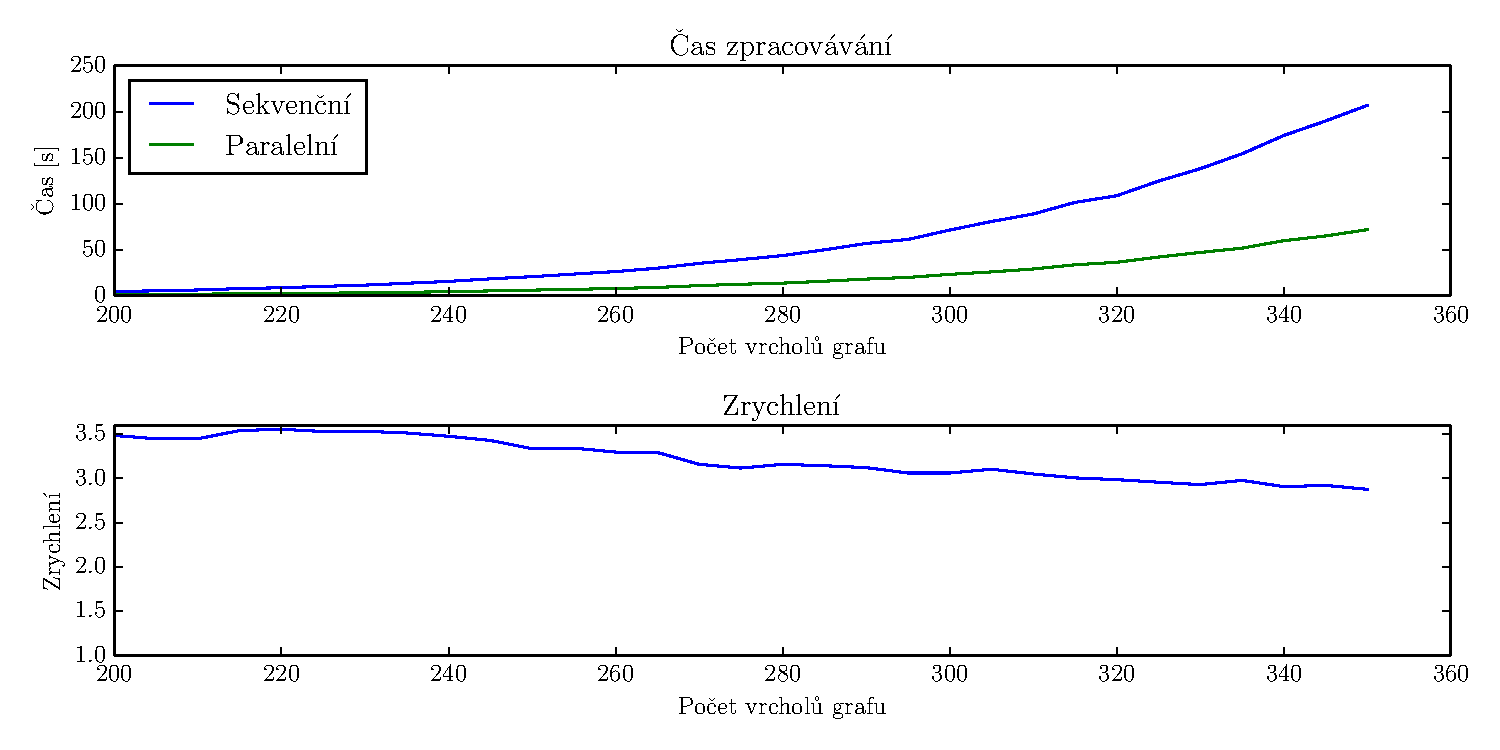
\includegraphics[scale=0.55]{images/5.pdf}}\\
    \subfloat[$60\,\%$ hran]{ 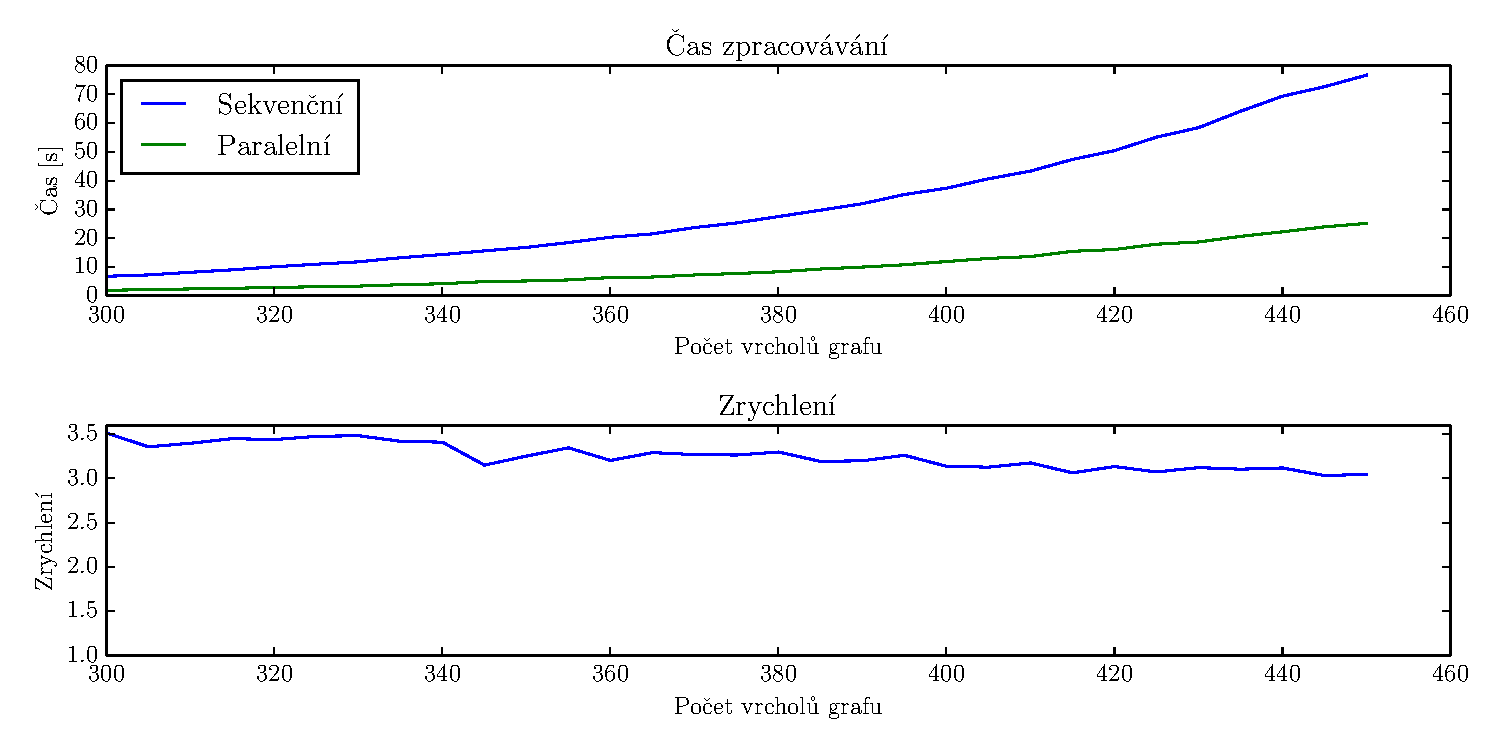
\includegraphics[scale=0.55]{images/6.pdf}}\\
    \subfloat[$70\,\%$ hran]{ 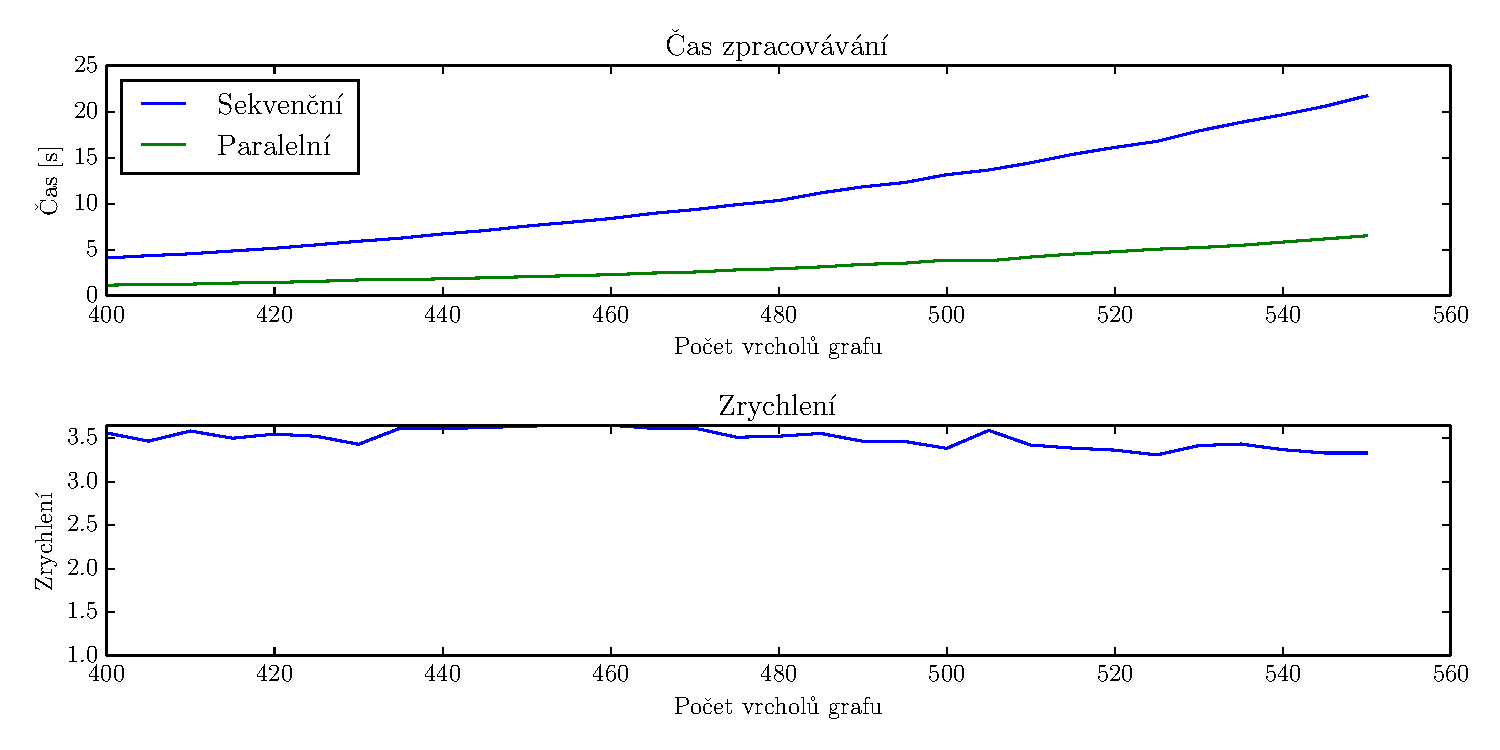
\includegraphics[scale=0.55]{images/7.pdf}}
    \caption{Naměřené výsledky rychlosti hledání maximálních nezávislých množin a zrychlení oproti sekvenčnímu algoritmu. Grafy obsažené v jednom grafu obsahují stejné procento všech hran.} \label{fig:SpeedResults}
\end{figure}


\section{Závěr}

\begin{thebibliography}{99}
\bibitem{demel} TODO demel
\end{thebibliography}

\appendix
\section{Použití programu} \label{appendix:ProgramUsage}

\section{Naměřené výsledky} \label{appendix:RawResults}

\begin{table}[H]
\begin{center}
\rowcolors{2}{lightgray}{white}
\begin{tabular}{ c c c c c }
\toprule
Vrcholů & Hran & Sekvenční [s] & Parelelní [s] & Zrychlení\\\midrule
200 & 9950 & 4.806 & 1.379 & 3.484\\
205 & 10455 & 5.457 & 1.583 & 3.446\\
210 & 10972 & 6.417 & 1.862 & 3.447\\
215 & 11502 & 7.905 & 2.233 & 3.539\\
220 & 12045 & 8.834 & 2.486 & 3.554\\
225 & 12600 & 10.320 & 2.926 & 3.528\\
230 & 13167 & 11.675 & 3.307 & 3.531\\
235 & 13747 & 13.686 & 3.897 & 3.512\\
240 & 14340 & 15.704 & 4.519 & 3.475\\
245 & 14945 & 18.481 & 5.391 & 3.428\\
250 & 15562 & 20.852 & 6.254 & 3.334\\
255 & 16192 & 23.675 & 7.085 & 3.341\\
260 & 16835 & 26.377 & 8.003 & 3.296\\
265 & 17490 & 30.030 & 9.123 & 3.292\\
270 & 18157 & 35.272 & 11.169 & 3.158\\
275 & 18837 & 39.345 & 12.627 & 3.116\\
280 & 19530 & 43.736 & 13.849 & 3.158\\
285 & 20235 & 49.988 & 15.907 & 3.142\\
290 & 20952 & 56.912 & 18.233 & 3.121\\
295 & 21682 & 61.219 & 20.003 & 3.060\\
300 & 22425 & 71.425 & 23.343 & 3.060\\
305 & 23180 & 80.738 & 26.021 & 3.103\\
310 & 23947 & 88.890 & 29.152 & 3.049\\
315 & 24727 & 101.445 & 33.761 & 3.005\\
320 & 25520 & 108.687 & 36.410 & 2.985\\
325 & 26325 & 124.581 & 42.150 & 2.956\\
330 & 27142 & 138.036 & 47.123 & 2.929\\
335 & 27972 & 154.214 & 51.808 & 2.977\\
340 & 28815 & 174.083 & 59.911 & 2.906\\
345 & 29670 & 189.836 & 65.013 & 2.920\\
350 & 30537 & 206.761 & 71.886 & 2.876\\
\bottomrule
\end{tabular}
\end{center}
\caption{Naměřené výsledky pro grafy s $50\,\%$ hran} 
\end{table}

\begin{table}[H]
\begin{center}
\rowcolors{2}{lightgray}{white}
\begin{tabular}{ c c c c c }
\toprule
Vrcholů & Hran & Sekvenční [s] & Parelelní [s] & Zrychlení\\\midrule
300 & 26910 & 6.805 & 1.938 & 3.511\\
305 & 27816 & 7.280 & 2.169 & 3.356\\
310 & 28737 & 8.192 & 2.413 & 3.396\\
315 & 29673 & 9.049 & 2.624 & 3.448\\
320 & 30624 & 10.111 & 2.942 & 3.437\\
325 & 31590 & 11.002 & 3.167 & 3.474\\
330 & 32571 & 11.819 & 3.395 & 3.481\\
335 & 33567 & 13.254 & 3.878 & 3.418\\
340 & 34578 & 14.360 & 4.213 & 3.408\\
345 & 35604 & 15.617 & 4.960 & 3.149\\
350 & 36645 & 16.846 & 5.182 & 3.251\\
355 & 37701 & 18.513 & 5.536 & 3.344\\
360 & 38772 & 20.369 & 6.360 & 3.202\\
365 & 39858 & 21.536 & 6.546 & 3.290\\
370 & 40959 & 23.727 & 7.260 & 3.268\\
375 & 42075 & 25.338 & 7.765 & 3.263\\
380 & 43206 & 27.552 & 8.358 & 3.297\\
385 & 44352 & 29.760 & 9.326 & 3.191\\
390 & 45513 & 32.013 & 10.009 & 3.198\\
395 & 46689 & 35.218 & 10.803 & 3.260\\
400 & 47880 & 37.397 & 11.926 & 3.136\\
405 & 49086 & 40.661 & 13.008 & 3.126\\
410 & 50307 & 43.336 & 13.655 & 3.174\\
415 & 51543 & 47.390 & 15.475 & 3.062\\
420 & 52794 & 50.443 & 16.103 & 3.133\\
425 & 54060 & 55.128 & 17.948 & 3.072\\
430 & 55341 & 58.416 & 18.720 & 3.121\\
435 & 56637 & 64.123 & 20.668 & 3.103\\
440 & 57948 & 69.349 & 22.250 & 3.117\\
445 & 59274 & 72.653 & 23.972 & 3.031\\
450 & 60615 & 76.661 & 25.176 & 3.045\\
\bottomrule
\end{tabular}
\end{center}
\caption{Naměřené výsledky pro grafy s $60\,\%$ hran} 
\end{table}

\begin{table}[H]
\begin{center}
\rowcolors{2}{lightgray}{white}
\begin{tabular}{ c c c c c }
\toprule
Vrcholů & Hran & Sekvenční [s] & Parelelní [s] & Zrychlení\\\midrule
400 & 55860 & 4.118 & 1.156 & 3.561\\
405 & 57267 & 4.361 & 1.258 & 3.466\\
410 & 58691 & 4.567 & 1.275 & 3.583\\
415 & 60133 & 4.875 & 1.393 & 3.500\\
420 & 61592 & 5.169 & 1.457 & 3.547\\
425 & 63069 & 5.538 & 1.572 & 3.522\\
430 & 64564 & 5.929 & 1.729 & 3.430\\
435 & 66076 & 6.263 & 1.731 & 3.617\\
440 & 67606 & 6.720 & 1.862 & 3.610\\
445 & 69153 & 7.085 & 1.956 & 3.623\\
450 & 70717 & 7.570 & 2.081 & 3.638\\
455 & 72299 & 7.977 & 2.185 & 3.650\\
460 & 73899 & 8.391 & 2.299 & 3.650\\
465 & 75516 & 8.952 & 2.478 & 3.613\\
470 & 77150 & 9.362 & 2.589 & 3.616\\
475 & 78802 & 9.900 & 2.819 & 3.511\\
480 & 80472 & 10.345 & 2.936 & 3.523\\
485 & 82159 & 11.172 & 3.143 & 3.555\\
490 & 83863 & 11.838 & 3.417 & 3.465\\
495 & 85585 & 12.301 & 3.552 & 3.463\\
500 & 87325 & 13.155 & 3.888 & 3.383\\
505 & 89082 & 13.664 & 3.806 & 3.590\\
510 & 90856 & 14.445 & 4.222 & 3.421\\
515 & 92648 & 15.364 & 4.538 & 3.386\\
520 & 94458 & 16.111 & 4.790 & 3.363\\
525 & 96285 & 16.770 & 5.069 & 3.308\\
530 & 98129 & 17.903 & 5.243 & 3.415\\
535 & 99991 & 18.835 & 5.486 & 3.433\\
540 & 101871 & 19.660 & 5.838 & 3.368\\
545 & 103768 & 20.578 & 6.180 & 3.330\\
550 & 105682 & 21.710 & 6.519 & 3.330\\
\bottomrule
\end{tabular}
\end{center}
\caption{Naměřené výsledky pro grafy s $70\,\%$ hran} 
\end{table}

\end{document}
